\documentclass{llncs}
\usepackage{paralist}
\usepackage{enumerate}
\usepackage[margin=1.3in]{geometry}
\usepackage[T1]{fontenc}
\usepackage{graphicx}

\begin{document}


\title{Visualization of Traffic in Los Angeles County Freeways}

\author{Kalyanee Chendke, Abhinand Kadavigere Ravikumar}

\institute{Viterbi School of Engineering, University of Southern California, Los Angeles, CA, United States}
\maketitle

\begin{abstract}

This paper presents a visualization of traffic data in Los Angeles county. The motivation behind this visualization is to geographically show the various parameters associated with traffic such as speed and congestion. Also, traffic congestion is a major problem in Los Angeles, and this project aims to visualize different metrics and trends. The dataset ssociated with the project is sufficiently detailed and could be used to identify the metrics and trends in the traffic flow. This paper lists the different visualizations that were used and also the possible uses of those to city planners and people so that they can plan their journeys better. 

\end{abstract}

\section{Introduction}\label{sec:Introduction}

The project is a web-based, interactive visualization of the Los Angeles county traffic data that was obtained in the months from January to March 2014. The visualization shows the presence of highway loop detectors across various freeways in Los Angeles. Each sensor is capable of recording vehicular flow information such as speed and volume. Such parameters were aggregated over each of the 3 months. For each sensor and for each month, the parameters measured were:
\begin{enumerate}
\item Speed: Average speed (in mph)
\item Volume: Average number of vehicles
\item Occupancy: Percentage of the time period (30s) the sensor is occupied 
\end{enumerate}

\subsection{Highway Loop Detectors}\label{sec:Highway Loop Detectors}

The data used for this project was taken from highway loop detectors \cite{inductionloopwiki}. Highway loop detectors use moving magnets to induce an electrical current to a nearby wire. Induction loops are used for transmission and reception of communication signals or for detection of metal objects in metal detectors or vehicle presence indicators. These detectors are usually present at the entrance and the exit of the freeways and the data that they recorded has been visualized.

\subsection{Data Aggregation and Visualization}\label{sec:Data Aggregation and Visualization}

The data was in a format which was not amenable for a web-based, interactive visualization. Hence, the various parameters mentioned above were aggregated using Python and collated into a JSON (JavaScript Object Notation) format. Each sensor was visualized as a circle on a freeway on a map, with the radius and the color being governed by occupancy and speed respectively.

The visualization itself was performed using d3.js and Leaflet. d3.js is a Javascript library for manipulating documents based on data \cite{d3website} \cite{Murray2013}. This tool is based on the landmark paper on Data Driven Documents by Mike Bostock \cite{MichaelBostock2011}. Map visualization was performed using Leaflet \cite{leafletwebsite}, a d3-based visualization toolkit for interactive maps.

\section{Dataset}\label{sec:Dataset}

\subsection{Data}\label{sec:Data}

The total size of the dataset was about 35GB. It was obtained using highway loop detectors on 44 different highways around the Los Angeles area, from the period of January to March 2014. The dataset contained 2 configuration files which explain the various fields contained in the actual data. The actual data consists of one file containing information about each of the sensors, and 3 other files consisting of readings of the various sensors, in no particular order.

The first configuration file ("hw\_fields.txt") contains: 

\begin{enumerate}
\item LINK\_ID: sensor id,
\item CONFIG\_ID: configuration id, 
\item OCCUPANY: the percentage of time between every 30s that the sensor was occupied and in use,
\item VOLUME: count of cars in time period of 30s,
\item SPEED: average speed of caes in time period of 30s, 
\item HOV\_SPEED not used,
\item LINK\_STATUS: OK if sensor is working fine
\end{enumerate}

The second configuration file ("hw\_config\_fields.txt") contains:

\begin{enumerate}
\item ONSTREET: highway name, e.g., 405, 
\item FROMSTREET: from exit
\item TOSTREET: to exit
\item START\_LAT\_LONG: sensor lat/long
\end{enumerate}

We have ignored the FROMSTREET and TOSTREET columns.
\newline
The sensor reading are in the format: 
\newline
\\ \indent \indent 82 | Caltrans-D12 | 01/06/2014 10:00 | 1201941 | 0 | 25 | 1 | 113 | OK
\\This sample is present for each sensor reading - where each field corresponds to CONFIG\_ID, AGENCY, data and time in 'MM/DD/YYYY HH24:MI' format, LINK\_ID, OCCUPANCY, SPEED, VOLUME, HOVSPEED and LINK\_STATUS respectively. For the purposes of visualization in this project, sensors whose link\_status was not OK or if the sensor had failed then their readings were ignored. 
\\ The sensor took those readings for every 30s, every day during this time period and recorded them. The speed, volume and occupancy is an average over 30s. Also, there were some readings for which certain values were missing. Hence, even those readings were ignored. 

\subsection{Pre Processing and Extraction}\label{sec:Pre Processing and Extraction}

Aggregation and collation of the data was a complex process considering the sheer volume of the data and the amount of processing required. Data was first understood by extracting small amounts using shell scripts. Python was then used to collect the parameters for each sensor and take averages for each month. Hence, data was merged from multiple data files (as the sensor data was present in random order over 3 files)  into a single JSON file.

\subsection {Data Structure}\label{sec:Data Structure}
The JSON file was written in the form such that it grouped all the attributes of a particular sensor together. 

The sensor-data2.json file that we generated is in the following format:

\{
\\ \indent ``1205297" :
\\ \indent ``params"  :
\\ \indent \indent  \{``02" :  \{"Vol": 34.11, "occ": 9.56, "speed": 53.52\},
\\ \indent \indent  ``03": \{"vol": 36.42, "occ": 9.21, "speed": 56.80\}, 
\\ \indent \indent   ``01": \{"vol": 33.86, "occ": 9.64, "speed": 52.79\}\}, 
\\ \indent    ``highway": ``5", 
\\ \indent ``coordinates": [-117.86918, 33.770044]
\\ \indent \}

This format enabled the visualization library in quick retrieval of the data. The key for this dictionary is the sensor ID. For each sensor ID, the Volume, Occupancy and Speed were aggregated on a per month basis. In this case, "01" corresponds to January, "02" to February and "03" to March. Lastly, the coordinates identified the location of each sensor.

Another JSON file that was used is the params5.json file:

\{
\\ \indent ``1205297": 
\\ \indent \{``02": 
\\ \indent \indent \{``03": [],
\\ \indent \indent  ``09": [\{``speed": 67, ``time": "10"\}, \{``speed": 60, ``time": ``11"\}, 
\\ \indent \indent  \indent \{``speed": 64, ``time": ``12"\}]
\\ \indent \indent \}
\\ \indent \}
\\ \}

The JSON file has been organized to get the values of the speeds on particular days of the month- the first Mondays and first Fridays (E.g: 02/03 and 02/09), considering those are the peak days of commute. For each sensor, the data is arranged per month and then per day. This file also has the time stamp for each instance of speed to indicate when the data was recorded. This file has been used for making the line graph. 

\section{Visualization}\label{sec:Visualization}

This web based visualization has been made keeping in mind the different attributes of the dataset. A user can select the appropriate highway and the month for which he wants to view data. 

\subsection {Plotting speed, volume and occupancy}\label{sec:Plotting speed, volume and occupancy}

Speed and volume has been plotted on the map using circles. Each circle represents a sensor on the highway. The higher the radius of the circle, the more is the volume recorded. In this case, high volume represents high traffic. Speed has also been shown on the same point by using color codes. A bluer color corresponds to a lower speed and a redder color corresponds to a higher speed. A user can hover over the points to see the exact values of speed and volume. Circles were chosen instead of paths as the sensors are randomly arranged in data, and the primary motivation is sensor data visualization and not route mapping. 
The occupancy is shown using a pie chart on each of the freeways. Each highway is provided with a marker. Every time a marker is hovered upon, a pie chart shows up which depicts the percentage of the time the sensor was occupied, and the highway name. 
The line chart shows the speed on various days of the week- on the first Mondays and first Fridays during different hours of the day. In this way, a user can get a better idea about which highway is congested the most and at what time (e.g. rush hour traffic on Monday mornings, less traffic during afternoon)

%\subsection {Plotting Trends}\label{sec:Trends}

% Overall it was observed that the speed is low during the non-peak hours of the day. Also, we realized that during rush hours, the traffic generally move slowly because of the commute. We inferred that the speed is high during the day during non-rush hours. This could be mainly because the traffic flow is smooth, and less volume of vehicles. The speed could also be affected by any accidents/incidents that happen during the day.  

\section{Design Decisions}\label{sec:Design}

\subsection {Visualization Wheel}\label{sec:Visualization Wheel}

\begin{figure}[h!]
	\centering
   \vspace{-10pt}
	 \hspace*{-0.5in}
   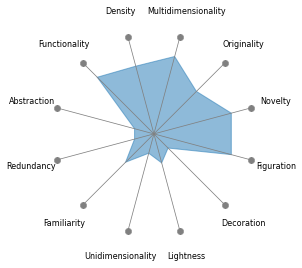
\includegraphics[scale=0.5]{vis_wheel.png}
   \caption{Cairo's Visualization wheel}
   \label{fig:cclogo}
\end{figure}



The visualization focuses on the upper half of the Cairo's wheel. It has been built based on the design principles of Cairo's wheel \cite{Cairo2012}. The visualization is highly figurative. It shows the different sensors on the LA map properly instead of abstracting them in a matrix or a similar form. This helps the user to get a good overview of the overall data so that he can drill down and know more about detailed data points, making it multi-dimensional. Also, the visualization is highly functional instead of being decorative. It does not contain any irrelevant content. 

\subsection {Semantic Pattern Mapping}\label{sec:Semantic Pattern}

The visualization has incorporated certain semantics \cite{Ware2008} to make it easier for the viewer to understand the mapping. The size of the sensor points has been varied to indicate the change in its magnitude- which in this case is represented by volume. The visualization has been partitioned to show hierarchy between the different elements. The map provides a high level overview and the line graph gives detailed drilled down showing the relationship of speed vs time for each sensor. The different layers used help to pre-attentively process the data so a user can identify the geography of a region very easily. The colors of the map correspond to the conventional colors used to represent the geographical areas.

\subsection {Mapping and Layers}\label{sec:Mapping and Layers}
There are three layers used with the project such that the data is visible easily. These include- the OpenStreetMap layer, stamen layer and the mapnik layer. These layers enhance the way the map is represented and are used to visualize the data better. The visualization was restrained by the way the dataset was obtained. The dataset does not contain contiguous points of sensors, they have been arranged randomly. Hence it is impossible to judge if points form a single contiguous path. Instead, there are circles as sensor points on the map. Also, in order to make the map less cluttered and more appealing for the viewer, panning and zooming has been used. It helps to focus on the particular area of interest. Furthermore, in order to understand the general trend of speed vs time for each sensor, these trends have been highlighted.

\section{Tools used}\label{sec:Tools}
D3.js provides multiple options to visualize data on a map. The Leaflet toolkit for interactive maps was chosen as it was the most user-friendly tool, along with the layers provided by Mapnik, OpenStreetMap and stamen. Leaflet also provided provision for having popups and information labels. Mapnik could also provide the same tools but those were harder to use. Python and bash shell scripting was used for data aggregation and collation. HTML and CSS provided the front-end of the website, and Javascript for scripting.

\section{Related Work}\label{sec: Related Work}
Similar work has been done on the web in the field of traffic visualization. At University of Southern California, Professor Cyrus Shahabi and his team have made a "Clearpath" app. Their application helps to find the best path such that the overall time to reach to a destination reduces and also the expenses of the travelers are thus saved. Another similar application is the "Waze" app. Waze app also works similarly by letting other vehicles know about the traffic flow in an area.

\section{Conclusion}\label{sec:Conclusion}

The main objective of the project was to be able to visualize the entire set of data available. The visualization has been made such that any novice reader can interpret the data easily. The visualization can be used by city planners such that the freeways could be designed well depending on the traffic conditions, or by novice readers planning his/her trips. We also concluded that the traffic congestion peaks during the early hours and also during the evening hours when people go to work. We realized that when the occupancy of a sensor was high, then the volume passing through the sensor was also high. Moreover, we learned to extract data that was in unstructured format initially and put it into a structured format. The website is located at \url{http://infovizgroup9.s3-website-us-west-1.amazonaws.com/html}

\section*{Acknowledgments}\label{sec:Acknowledgments}

The authors would like to thank Professor Luciano Nocera for his guidance and giving access to the data. The authors would also like to thank the critique group for their feedback which helped in improving the visualization.

\bibliographystyle{splncs03}
\bibliography{bibfile} 
\nocite{*}
\end{document}